\documentclass[a4paper,11pt]{article}

\usepackage{../préambule}

\begin{document}

\begin{center}
	{\tiny colle dans ton cahier d'exercices}
	
	\LARGE
	\myuline{Exercices : symétrie axiale}
	\vspace{1em}
\end{center}

\begin{attention}[frametitle={\hspace{0.35\textwidth}⚠ Attention ⚠}]
	\center Dessine au \textbf{crayon à papier} !
\end{attention}

\begin{exercice}
	\begin{enumerate}
		\item Donne une lettre à chaque point de la figure : A, B, C, D, E et F.
		\item Construit le symétrique de chacun de ces points par rapport à l'axe $(d)$.
		\item Complète la figure. \vspace{0.5em}
	\end{enumerate}
	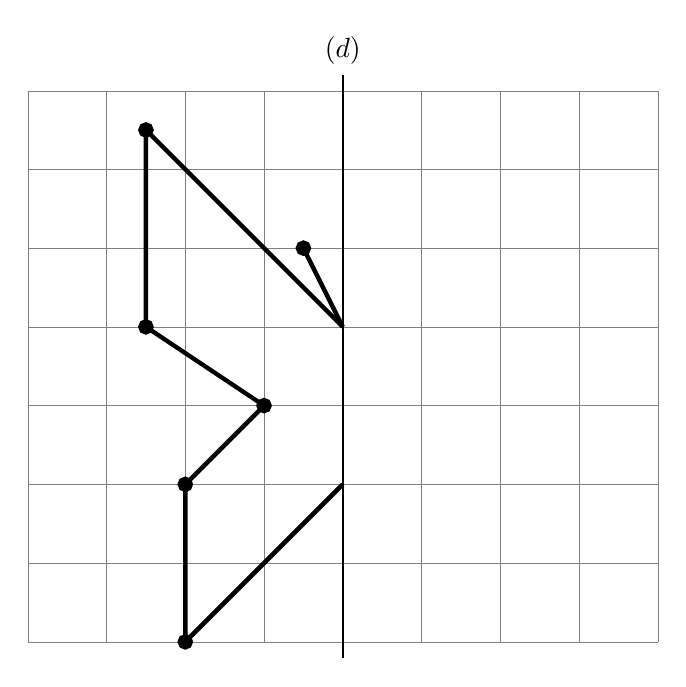
\begin{tikzpicture}[c/.style={insert path={circle[radius=2pt]},fill}]
		\draw[gray,ultra thin] (0,0) grid (8,7);
		\draw[black,thick] (4,-0.2) -- (4,7.2) node[anchor=south]{$(d)$};

		% corps
		\draw[black,ultra thick] (4,4)
		-- ++(-2.5,2.5) [c]
		-- ++(0,-2.5) [c]
		-- ++(1.5,-1) [c]
		-- ++(-1,-1) [c]
		-- ++(0,-2) [c]
		-- ++(2,2);
		% antenne
		\draw[black,ultra thick] (4,4) -- ++(-0.5,1) [c];

		% % corps
		% \draw[black,ultra thick] (4,4) [c] -- ++(2.5,2.5) [c] -- ++(0,-2.5) [c] -- ++(-1.5,-1) [c] -- ++(1,-1) [c] -- ++(0,-2) [c] -- ++(-2,2) [c];
		% % antenne
		% \draw[black,ultra thick] (4,4) -- ++(0.5,1) [c];
	\end{tikzpicture}

	Quelle figure obtient-on ? \vspace{2em}
\end{exercice}

\begin{exercice}
	Faire le symétrique de la figure ci-dessous par rapport à l'axe $(d)$ :

	(Essaie de faire partie par partie : d'abord le nez, puis les moustaches, puis les oreilles...)

	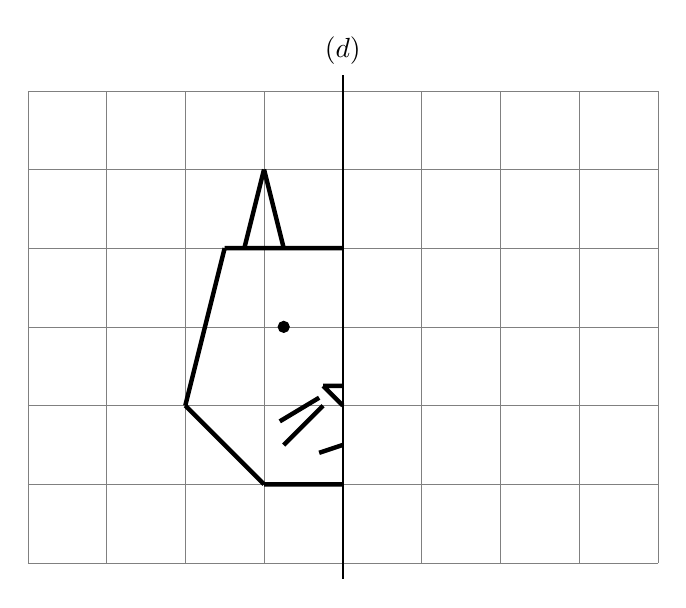
\begin{tikzpicture}[c/.style={insert path={circle[radius=0pt]},fill}]
		\draw[gray,ultra thin] (0,0) grid (8,6);
		\draw[black,thick] (4,-0.2) -- (4,6.2) node[anchor=south]{$(d)$};

		% head
		\draw[black,ultra thick] (4,1) -- ++(-1,0) [c] -- ++(-1,1) [c] -- ++(0.5,2) [c] -- ++(1.5,0);
		% ear
		\draw[black,ultra thick] (3.25,4) [c] -- ++(-0.25,1) [c] -- ++(-0.25,-1) [c];
		% nose
		\draw[black,ultra thick] (4,2) -- ++(-0.25,0.25) [c] -- ++(0.25,0);
		% eye
		\draw[black,fill] (3.25,3) circle (2pt);
		% mustache
		\draw[black,ultra thick] (3.75,2) -- ++(-0.5,-0.5);
		\draw[black,ultra thick] (3.7,2.1) -- ++(-0.5,-0.3);
		% mouth
		\draw[black,ultra thick] (4,1.5) -- ++(-0.3,-0.1);

		% \draw[black,ultra thick] (4,1) -- ++(1,0) [c] -- ++(1,1) [c] -- ++(-0.5,2) [c] -- ++(-1.5,0);
		% \draw[black,ultra thick] (4.75,4) [c] -- ++(0.25,1) [c] -- ++(0.25,-1) [c];
		% \draw[black,ultra thick] (4,2) -- ++(0.25,0.25) [c] -- ++(-0.25,0);
		% \draw[black,fill] (4.75,3) circle (2pt);
		% \draw[black,ultra thick] (4.25,2) -- ++(0.5,-0.5);
		% \draw[black,ultra thick] (4.3,2.1) -- ++(0.5,-0.3);
		% \draw[black,ultra thick] (4,1.5) -- ++(0.3,-0.1);
	\end{tikzpicture}

	Quelle figure obtient-on ? \vspace{2em}
\end{exercice}

\end{document}